\chapter{Process model}
\label{Process model}
Process models for software development is a representation of the process and the activities required for developing the software. In software engineering there is two different development methods, pland-driven and agile development. The plan-driven approach is based on sperate development stages and iterations can occur within the activities e.g. the implementation of the software. The agile approach the specification, design, implementation and tests are all iterated on as a whole. \citep{sommerville}

The process model is a meld of elements from both plan driven and agile development. The process is plan driven in so far as to include a clear goal of what the initial requirements of the system are. The process model is very agile in that, although there is a clear outline as to what the requirements are, these are incrementally approached, with a simple starting point becoming increasingly covering of the project vision through the subsequent increments. The reason the group approached this project with our 'own' process model is to better explain what we're actually doing, rather than forcing ourselves into picking a development method and try to explain what we're doing according to that method.

The increments will be split up into four sections. Initially some of the already known requirements will be considered from previous increments and for the first increment from the analysis chapter, and these requirements will be the topic of the increment.
After the initial requirement consideration, a design phase follows which details the design and problem considerations preceding the implementation. The design phase is then followed by an implementation phase which will explain the implementation process. The final phase is an evaluation of the increment and will concern whether the requirements were fulfilled, if an requirement needs to be altered, or if an requirement will be continued in the following increment. The evaluation will also include several tests of the implementation, in order to see what works and what doesn't work. The evaluated requirements from an increment will then become the starting point of the next increment. 

The process includes both pair programming and pair writing, which is to promote cooperation and attempt to avoid having a single individual involved in a task beyond their capabilities and to get a second opinion. This is also to ensure that information is quickly communicated and exchanged by group members. The process uses pair programming because it promotes better programming and is usually very motivating in socially engaging issues with cooperation of project members.


\begin{figure}[h]
	\centering
	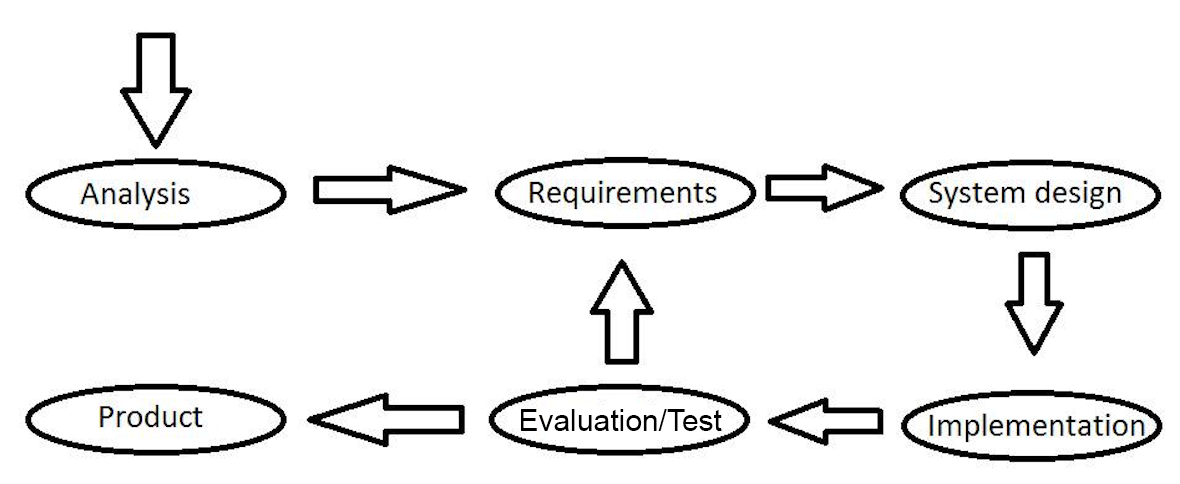
\includegraphics[scale=0.30]{billeder/process-model}
	\caption{Process model used for the project}
	\label{pm}
\end{figure}